\chapter{Hardware Design and Development of Aerial Robot Swarm Platforms}

\section{Generic Design}

\subsection{Components on the drone}

\subsubsection{Frame}
The choice of the drone frame is really important.
The size of the frame will impact the choice of the propellers, the motors, the \acrshort{esc} and the battery.
It has to be big enough to have enough space for all the components of the drone.
And, as the aim is to create a swarm of drone, the smaller the drone is the better.

\subsubsection{Props}
The propellers have three major characteristics. Their size, their pitch, and their number of blades.

The size of the propellers in part fixed by the size of the frame.

The higher the pitch the higher the thrust but also higher torque is needed from the motors.
Moreover, the pitch should always be less than 2/3 of the propeller size as higher pitch could cause air disturbances (Vortex Ring State).
So, the pitch was chosen by taking the highest pitch on the market that respected the 2/3 ratio.

The number of blades impact thrust and efficiency. More blades mean increased thrust but decreased efficiency.

The propeller specification are generally either \emph{SxPxB} or \emph{SSPPxB}.
S being the size, P the pitch and B the number of blades
(e.g. for a size of 70mm and pitch of 4.5 and 2 blades, 7x4.5x2 and 7045x2).

\subsubsection{Motors}
The motors have different characteristics. Its width, height and KV.

These characteristics are in part fixed by the frame and the propellers.

Some motors comes with propeller adapter.

\subsubsection{ESCs}
The ESC have to major characteristics, their current limit and their max voltage input in S unit,number of cell of LiPo battery (e.g. 3S).

The motor current consumption should never exceed the ESC current limit.

It is advise to buy extra spare esc and oversize them as it is a critical part of the drone.

\subsubsection{Battery}
The battery has a voltage fixed by its number of cells, $3.7V$ nominal per cell.
It has a capacity in mAh,
The current draw the LiPo can support is its capacity times the C-rating.

The motor current consumption should never exceed the maximum current draw of the LiPo.

\subsubsection{Power distribution board}
The PDB has a max current and max voltage that should not be exceeded.

\subsubsection{RC Receiver}
For a drone, the minimum amount of channel for a receiver is 6.
The receiver can either send to the flight controller the received signal via PWM or PPM.

\subsubsection{Flight Controller}
The flight controller is a electronic board with sensors (e.g. accelerometer, gyroscope, barometer…).

The choice of a flight controller often depends on the compatibility of the firmware wanted. For autonomous drone, the flight controller should be compatible with ArduPilot or PX4 and for racing, It should be compatible with Betaflight.

\subsubsection{Companion computer}
The companion computer on a drone has to be light and not take to much place (it is a major concern).

\subsubsection{WiFi module}
The WiFi module should be selected with the bandwidth required and it should be compatible with the companion computer.

\subsubsection{Cables and Connectors}
Some of the cables and connectors can come with the previous components but often some has to be bought.

It is an important step to verify that everything will be able to be connected to the other components.

\subsubsection{Attaching components}
Straps, screws, mounting tape and zip ties are used to attach the different components of the drone.

\subsubsection{Anti-vibration system}
It is important to reduce the vibration of the sensors on the drone to have accurate data.

\subsubsection{Low-voltage Alarm}
An alarm for low-voltage is important to avoid continuing to fly with an empty LiPo battery that could degrade and even catch fire.

\subsection{Components on the ground}

\subsubsection{RC Transmitter}
As told previously, an transmitter with 6 channels is enough for a drone. But to avoid, buying another transmitter for other projects that need more channel. It is interesting to buy a 8 or 10 channels transmitter.

\subsubsection{Battery Charger}
The battery charger has to be compatible with LiPo with the corresponding voltage.

\subsubsection{LiPo Fireproof Bag}
To recharge LiPo safely using a fireproof bag is a most.

\subsubsection{Propeller Balancer}
The Propeller Balancer is used to balance propeller to avoid vibrations.


\section{Specific Design of this Project}

\subsection{Detailed Quadrotor Hardware Requirements}
\begin{itemize}
    \item Thrust to weight ratio of at least 2
    \item Flight time > 5 minutes
    \item Smallest possible size to fit all components
    \item Has to carry an on-board computer with a powerful processor and enough RAM (4GB) and WiFi compatibility.
    \item Overall as durable as possible and protect the weaker components.
\end{itemize}

\subsection{Components on the drone}


This is a \cite{hackaday_navio} with RPi2 and Navio2.
Another project \cite{instructables_navio}.

\subsubsection{Frame}
It is F2 Mito \cite{bangood_f2_mito}.

It is 275mm frame in carbon fiber and it is big enough for the Jetson Nano.

It weights 125g.

\subsubsection{Props}
It is 5x3 propeller \cite{bangood_propeller}. The size is 5 inch it is the biggest propeller that would leave enough place for the Jetson Nano. The pitch is 30mm as higher pitch would increase Vortex Risk State. It has 2 blade as it is more efficient and thus less straining for the battery and motor. It is in plastic as it is more resistant to crash.

It weights 2g each so 8g total.

\subsubsection{Motors}
It is Emax RS2205 2300KV \cite{bangood_motor}. The size of 2205 and kv of 2300 is recommended to 5 inch propeller. The thrust with 5x3 propeller at 75\% is 614g with 7.54A consumption. So for a thrust/weight ratio of 2 the drone can weight $1228g=614g \times 4motor / 2$ \cite{google_sheets_motor}.

It weights 30g each so 120g total.

\subsubsection{ESCs}
It is 20A ESC \cite{bangood_esc} as they do not support higher amperage than their specification so a margin is taken. The motors for 7.54A each produce a total thrust of $2456g=614g\times 4motor$. 20A ESC are enough.

It weights 28g each so 112g total.

They are placed on the frame arms.

\subsubsection{Zip}
\cite{bangood_zip_ties}. It holds the ESC and other elements together.\\
Its dimensions are 3 x 100 mm.

\subsubsection{Battery}
Lipo 11.1V 1500mAh 40C XT60 Plug \cite{bangood_battery}. With $ \frac{1.5mAh \times 60min}{3A \times 4motor}= 7.5min$. It can also support a continuous current draw of $60A = 1.5mAh\times 40C$.

It weights 113g.

Its dimensions are 29.5 * 34 * 66 mm.

It is placed under the drone.

\subsubsection{Battery Straps}
\cite{bangood_battery_strap}. It is to hold the battery.

It should weight around 10g.

Its dimensions are 260 * 20 mm.

\subsubsection{Power distribution board}
Matek Mini Power \cite{bangood_pdb}. It support 3S battery. It can output 20A continuous max per ESC outputs. It has a BEC of 5V and 3A continuous so it can power the Jetson Nano without problem.

It weights 6g.

Its dimensions are 36 x 36 mm.

It is placed in the center of the frame. It is attached with the 4 standoff.

\subsubsection{XT60 connector cable}
\cite{bangood_xt60_cable}. It is to connect the battery to Power Distribution Board without cutting cable (it would use the female XT60 cable). The male XT60 would be used to power the Jetson Nano.

It should weights around 10g.

\subsubsection{RC Receiver}
Flysky 2.4G 6CH FS-iA6B \cite{bangood_receiver}. It has 6 channel. It is enough as we do not use RC much in this project.

It weights 15g.

Its dimensions are 47 x 26.2 x 15 mm.

It is placed at the rear of the drone zip tied.

\subsubsection{Dupont Cable Female to Female}
\cite{bangood_dupont_cable}. It is to connect the flight controller to the RC Receiver.

Its length is 10cm.

\subsubsection{Flight Controller}
\begin{description}
    \item[PixRacer] \cite{mrobotics_pixracer}. This flight controller is compatible with all firmware. It is from the PixHawk series that is used a lot so a lot of resources is available for it. All cable and connector needed are delivered with it. It will be powered with the ESC BEC.

          It weights 11g.

          Its dimensions are 36 x 36 mm.

          It is placed on top of the Power Distribution Board with standoff.

    \item[Navio2] \cite{emlid_navio2}. It is compatible with ArduPilot and PX4 not ROSflight. It is used coupled with a Raspberry Pi. All cable and connector needed are delivered with it. It will be powered with the power module \cite{emlid_power_module} provided with the Navio2. You have the response of Emlid about the hardware compatibility here \cite{emlid_rpi_compatibility}.

          It weights 23g.

          Its dimensions are 55 x 65 mm.

          It is placed on top of the Raspberry Pi.
\end{description}

\subsubsection{Companion computer}

\begin{description}
    \item[Jetson Nano] Already bought.

          It weights 136g.

          Its dimensions are 95.3 x 76.2 mm.

          It is placed on top of the drone with Kyosho Zeal under it to dampen vibration.

    \item[Raspberry Pi 4] It is powered with Navio2.

          It weights 50g.

          Its dimensions are 87 x 58.5 mm.

          It is placed on top of the drone.
\end{description}

\subsubsection{Anti-vibration}
\begin{description}
    \item[Anti-Vibration Standoff] \cite{bangood_standoff}. It dampens the vibration propagated to the PixRacer.
    \item[Kyosho Zeal] \cite{amazon_kyosho}. It dampens the vibration propagated to the Raspberry Pi by putting it under the Raspberry case.
\end{description}

\subsubsection{Wifi module}
300Mbps Wireless usb adapter \cite{amazon_panda_wifi_module}. It has 300 Mbps bandwidth so the router could support around 13 drones. The router has a bandwidth of 4000Mbps.

It weights 9g.

It is placed on a usb port of the Jetson Nano or the Raspberry Pi.

\subsubsection{XT60 to 2.1-5.5mm dc plug}
\cite{bangood_xt60_connector}. It is to power the Jetson Nano.

It should weights around 5g.

\subsubsection{Low-voltage Alarm}
\cite{bangood_battery_monitor}. It is to warn when the lipo battery is low as it could damage it to use it when it is discharged.

It weights 11g.

It is placed at the rear of the drone.

\subsection{Components on the ground}

\subsubsection{RC Transmitter}
Flysky i6X FS-i6X 2.4GHz 10CH \cite{bangood_transmitter}. It is compatible with the RC receiver. It has 10 channel that is 4 more than the receiver. It could be useful for future project with a need of more channel. Another RC transmitter would not have to be bought.

\subsubsection{Battery Charger}
\cite{bangood_battery_charger}. It is compatible with the battery.

\subsubsection{Propeller Balancer}
\cite{bangood_prop_balancer}. It is to balance propeller.

\subsubsection{Weight}
The total weight of the drone is around 700g.

\subsubsection{Simulation}
\begin{figure}[!ht]
    \centering
    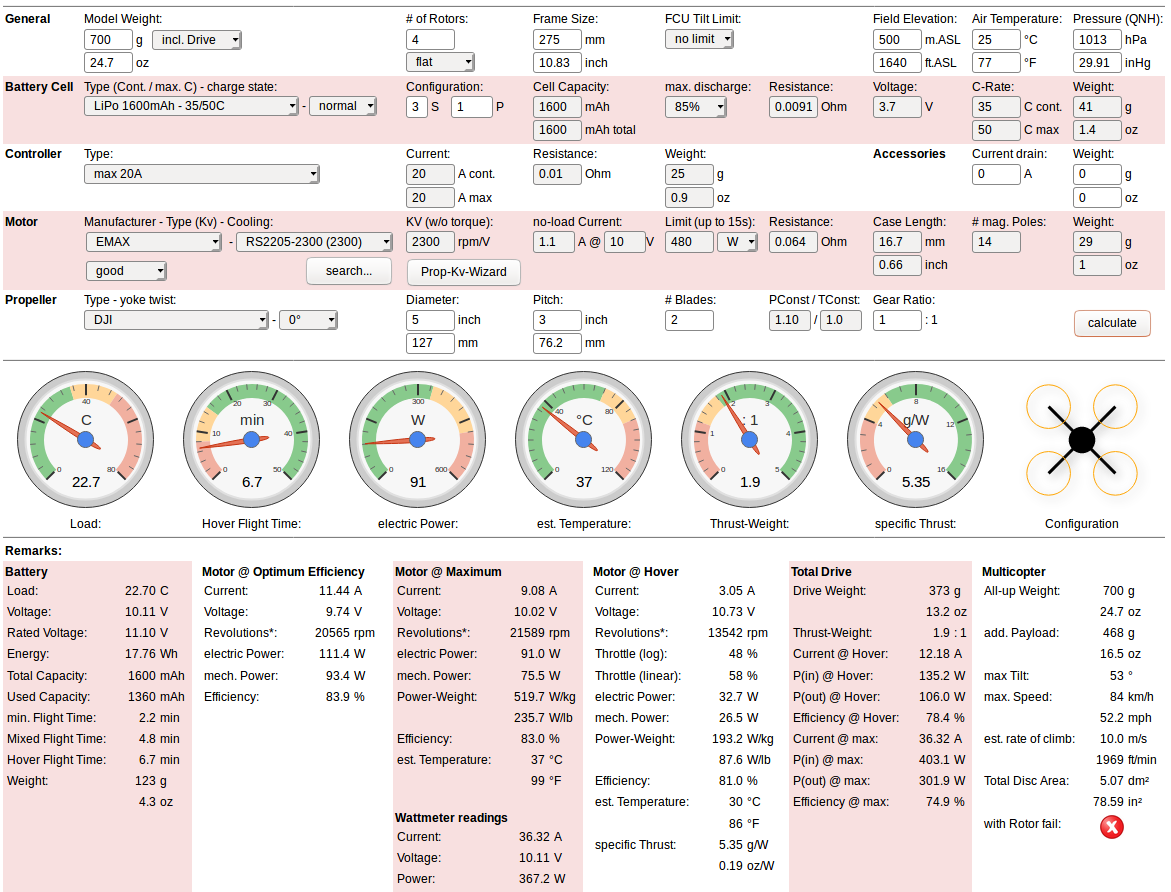
\includegraphics[width=\linewidth]{design/ecalc.png}
    \caption{eCalc copter simulation}
    \label{fig:ecalc}
\end{figure}
